\section{Sequential MNIST}

\subsection{Task and evaluation criteria}
The simple function task is a purely synthetic task, that doesn't require a deep network. As such it doesn't tests if an arithmetic layer prevents the networks ability to be optimized using gradient decent.

The sequential MNIST task, takes the numerical value of a sequence of MNIST digits and then applies a binary operation recursively. That is $t_i = Op(t_{i-1}, z_t)$, where $z_t$ is the MNIST digit's numerical value.

As the performance of this task depends on the quality of the image-to-scalar network, as well as the arithmetic layer itself. As threshold has to be determined from an empirical baseline. This is done by letting the arithmetic layer be solved, such that only the image-to-scalar is learned. By learning this over multiple seeds an an upper bound for an MSE threshold can be set. In our experiment we use the 1\% one-sided upper confidence-interval, assuming a student-t distribution.

A success-criteria is again used, as reporting the MSE is not interpretable, and models that don't converge will obscure the mean. Furthermore, because the operation is applied recursively, natural error from the dataset will accumulate over time, thus exponentially increasing the MSE. Using a baseline model and reporting the successfulness solves this issue.

\subsection{Without the \texorpdfstring{$\mathrm{R}_z$}{R\_z} regularizer}
\label{sec:appendix:sequential-mnist:ablation}

As an ablation study of just the $\mathrm{R}_z$ regularizer, figure \ref{fig:sequential-mnist-prod-ablation} shows the NMU and $\mathrm{NAC}_{\bullet,\mathrm{NMU}}$ models without the $\mathrm{R}_z$ regularizer. The success-rate is somewhat similar. However, as seen in the ``sparsity error'' plot, the solution is quite different.

\begin{figure}[h]
\centering
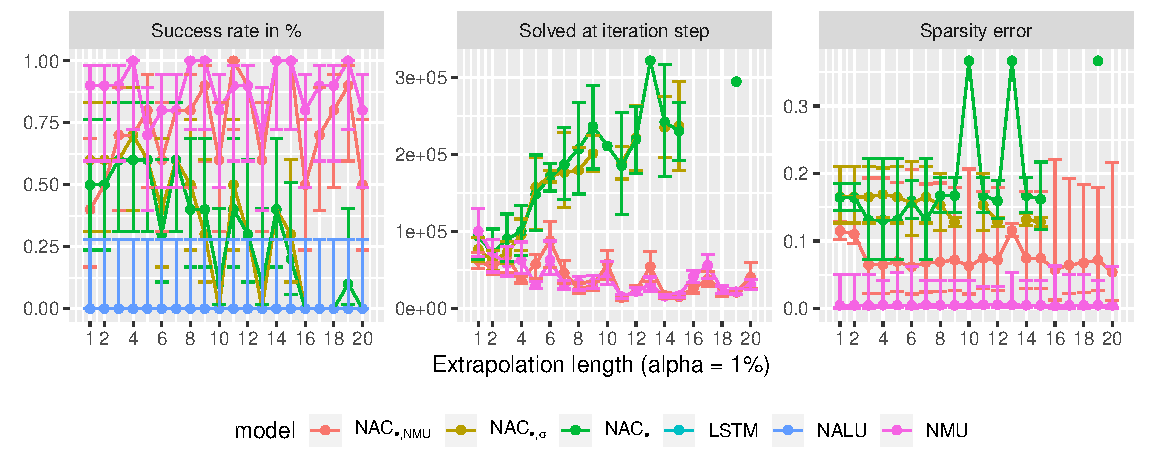
\includegraphics[width=\linewidth,trim={0 0.5cm 0 0},clip]{results/sequential_mnist_prod_long_ablation.pdf}
\caption{Shows the ability of each model to backpropergation and extrapolate to larger sequence lengths. The NMU and $\mathrm{NAC}_{\bullet,\mathrm{NMU}}$ models do not use the $\mathrm{R}_z$ regularizer.} 
\label{fig:sequential-mnist-prod-ablation}
\end{figure}
